\documentclass[a4paper,12pt]{extarticle}
\usepackage[utf8x]{inputenc}
\usepackage[T1,T2A]{fontenc}
\usepackage[russian]{babel}
\usepackage{hyperref}
\usepackage{indentfirst}
\usepackage{listings}
\usepackage{color}
\usepackage{here}
\usepackage{array}
\usepackage{multirow}
\usepackage{graphicx}

\usepackage{caption}
\renewcommand{\lstlistingname}{Программа} % заголовок листингов кода

\bibliographystyle{ugost2008ls}

\usepackage{listings}
\lstset{ %
extendedchars=\true,
keepspaces=true,
language=C,						% choose the language of the code
basicstyle=\footnotesize,		% the size of the fonts that are used for the code
numbers=left,					% where to put the line-numbers
numberstyle=\footnotesize,		% the size of the fonts that are used for the line-numbers
stepnumber=1,					% the step between two line-numbers. If it is 1 each line will be numbered
numbersep=5pt,					% how far the line-numbers are from the code
backgroundcolor=\color{white},	% choose the background color. You must add \usepackage{color}
showspaces=false				% show spaces adding particular underscores
showstringspaces=false,			% underline spaces within strings
showtabs=false,					% show tabs within strings adding particular underscores
frame=single,           		% adds a frame around the code
tabsize=2,						% sets default tabsize to 2 spaces
captionpos=t,					% sets the caption-position to top
breaklines=true,				% sets automatic line breaking
breakatwhitespace=false,		% sets if automatic breaks should only happen at whitespace
escapeinside={\%*}{*)},			% if you want to add a comment within your code
postbreak=\raisebox{0ex}[0ex][0ex]{\ensuremath{\color{red}\hookrightarrow\space}},
texcl=true,
inputpath=listings,                     % директория с листингами
}

\usepackage[left=2cm,right=2cm,
top=2cm,bottom=2cm,bindingoffset=0cm]{geometry}

%% Нумерация картинок по секциям
\usepackage{chngcntr}
\counterwithin{figure}{section}
\counterwithin{table}{section}

%%Точки нумерации заголовков
\usepackage{titlesec}
\titlelabel{\thetitle.\quad}
\usepackage[dotinlabels]{titletoc}

%% Оформления подписи рисунка
\addto\captionsrussian{\renewcommand{\figurename}{Рисунок}}
\captionsetup[figure]{labelsep = period}

%% Подпись таблицы
\DeclareCaptionFormat{hfillstart}{\hfill#1#2#3\par}
\captionsetup[table]{format=hfillstart,labelsep=newline,justification=centering,skip=-10pt,textfont=bf}

%% Путь к каталогу с рисунками
\graphicspath{{fig/}}

%% Внесение titlepage в учёт счётчика страниц
\makeatletter
\renewenvironment{titlepage} {
 \thispagestyle{empty}
}
\makeatother


\begin{document}	% начало документа

% Титульная страница
\begin{titlepage}	% начало титульной страницы

	\begin{center}		% выравнивание по центру

		\large Санкт-Петербургский Политехнический Университет Петра Великого\\
		\large Институт компьютерных наук и технологий \\
		\large Кафедра компьютерных систем и программных технологий\\[6cm]
		% название института, затем отступ 6см
		
		\huge Базы данных\\[0.5cm] % название работы, затем отступ 0,5см
		\large Отчет по лабораторной работе №1\\[0.1cm]
		\large Разработка структуры БД\\[5cm]

	\end{center}


	\begin{flushright} % выравнивание по правому краю
		\begin{minipage}{0.25\textwidth} % врезка в половину ширины текста
			\begin{flushleft} % выровнять её содержимое по левому краю

				\large\textbf{Работу выполнил:}\\
				\large Графов Д.И.\\
				\large {Группа:} 33531/2\\
				
				\large \textbf{Преподаватель:}\\
				\large Мяснов А.В.

			\end{flushleft}
		\end{minipage}
	\end{flushright}
	
	\vfill % заполнить всё доступное ниже пространство

	\begin{center}
	\large Санкт-Петербург\\
	\large \the\year % вывести дату
	\end{center} % закончить выравнивание по центру

\thispagestyle{empty} % не нумеровать страницу
\end{titlepage} % конец титульной страницы

\vfill % заполнить всё доступное ниже пространство


% Содержание
% Содержание
\renewcommand\contentsname{\centerline{Содержание}}
\tableofcontents
\newpage



\section{Техническое задание}
\subsection{Терминология}
Сервер, серверная часть – совокупность скриптов и СУБД, работающих на сервере сервиса. Бэкенд.

Клиентская часть, клиент, приложение – любое стороннее приложение (в данном случае имеется в виду Web-приложение), взаимодействующее с данными сервиса посредством REST API методом отсылки запросов в серверную часть и получения от нее результатов.

CRUD — акроним, обозначающий четыре базовые функции, используемые при работе с базами данных: создание (англ. create), чтение (read), модификация (update), удаление (delete).
\subsection{Постановка задачи}
Необходимо разработать клиент-серверное приложение для осуществелния CRUID операций с таблицой drinks из базы данных (БД) wine\_card. В качестве основого языка использовать JavaScript.

Платформой серверной части должна стать Node или Node.js — программная платформа, основанная на движке V8 (транслирующем JavaScript в машинный код).

В качестве сервера стоит использовать сервис, написанный с помощью Express - одного из самых популярных легковесных фреймворков, используемых при создании веб-приложений для node.
На серверной части должно быть осуществлено подключение к БД wine\_card посредством СУБД PostgreSQL и библиотеки Sequelize.

Клиентская часть должна представлять из себя одностраничное Web-приложение, написанное на Vue.js.

После нажатия на большую кпопку "V" пользователь получает таблицу со всеми напитками, расположенными в базе wine\_card. 
Получив таблицу, пользователь может получить информацию о напитке: его название, рейтинг, объём, крепкость, среднюю цену и тип напитка; изменить существующую запись, удалить её, или добавить новую.
Также, после нажатия на элемент таблицы, отображается информация о том, из каких компонентов состоит напиток, а также о том, в каких барах имеется данный напиток.

\subsection{Общение клиента с сервером}
Общение клиента с сервером осуществлять через http-запросы к /api/ с передачей соответствующих атрибутов.
При получении запроса, сервер должен осуществлять соответствующий запрос к СУБД. Далее, если http-запрос является get-запросом, сервер должен отправлять клиенту ответ в формате JSON. Если же это post или delete-запрос, то текстовое сообщение о статусе операции.

\newpage
\section{Программа работы}
\begin{enumerate}
	\item Выбор темы курсовой работы.
	\item Написание и согласование технического задания по курсовой работе с подробным описанием реализуемой функциональности.
	\item Реализация всей требуемой функциональности.
	\item Тестирование корректности работы.
	\item Демонстрация результатов преподавателю.
	\item Оформление отчета по курсовой работе.
\end{enumerate}

\section{Реализация}
Со всем исходным кодом приложения можно ознакомиться по адресу:

\href{http://gitlab.icc.spbstu.ru/grafa/wine_card/cource}{http://gitlab.icc.spbstu.ru/grafa/wine\_card/cource}.
\subsection{Backend}
Для написания серверной части была использована библиотека Express.js и Sequelize.js.

Для дальнейших взаимодействий с СУБД посредстам библиотеки Sequelize в директории /models были созданы JS-представления таблиц из БД wine\_card.

Серверная часть приложения содержит 6 возможных эндпоинтов. (см. листинг 1).

\begin{itemize}
	\item /api/all\_drinks - сервер получает get-запрос, чтобы получить все напитки из таблицы drinks. Обратившись к СУБД, сервер массив объектов в формате json, содержащий всевозможную информацию о напитках.(см. листинг 1, строки 23-29)
	
	Пример возвращаемого объекта:
\begin{lstlisting}
{
	"drink_id": 1,
	"title": "боярский",
	"rating": 9.2,
	"volume": 100,
	"alcohol": 20,
	"average_price": 200,
	"drink_type": "шоты"
}\end{lstlisting}
	\item /api/components - по get-запросу с атрибутом drink\_id сервер обращается к СУБД и возвращает список компонентов данного напитка. Для того, чтобы получить список компонентов, делается запрос к смежной таблице drinks\_components, оттуда берётся component\_id и по нему ищется вся нужная информация. (см. листинг 1, строки 31-39)
	\item /api/places - по get-запросу с атрибутом drink\_id сервер обращается к СУБД и возвращает список мест, где можно выпить данный напиток. (см. листинг 1, строки 41-49)
	\item /api/edit\_drink - по post-запросу c атрибутами [drink\_id, title, rating, volume, alcohol, average\_price, drink\_type] сервер обращается к СУБД и изменяет существующую запись в таблице. (см. листинг 1, строки 74-80)
	\item /api/delete\_drink - по delete-запросу c атрибутом drink\_id сервер обращается к СУБД и удаляет существующую запись в таблице. (см. листинг 1, строки 82-100)
	\item /api/new\_drink по post-запросу c атрибутами [drink\_id, title, rating, volume, alcohol, average\_price, drink\_type] сервер обращается к СУБД и добавляет новую запись в таблицу.
\end{itemize}

\lstinputlisting[
caption={Исходный код api.js},
]{../../routes/api.js}

\subsection{Frontend}
Для проектирования пользовательского интерфейса была использована библиотека Vue.js, был написан компонент drinks, который и представляет из себя главную (единственную) страницу web-приложения:

\begin{figure}[H]
	\begin{center}
		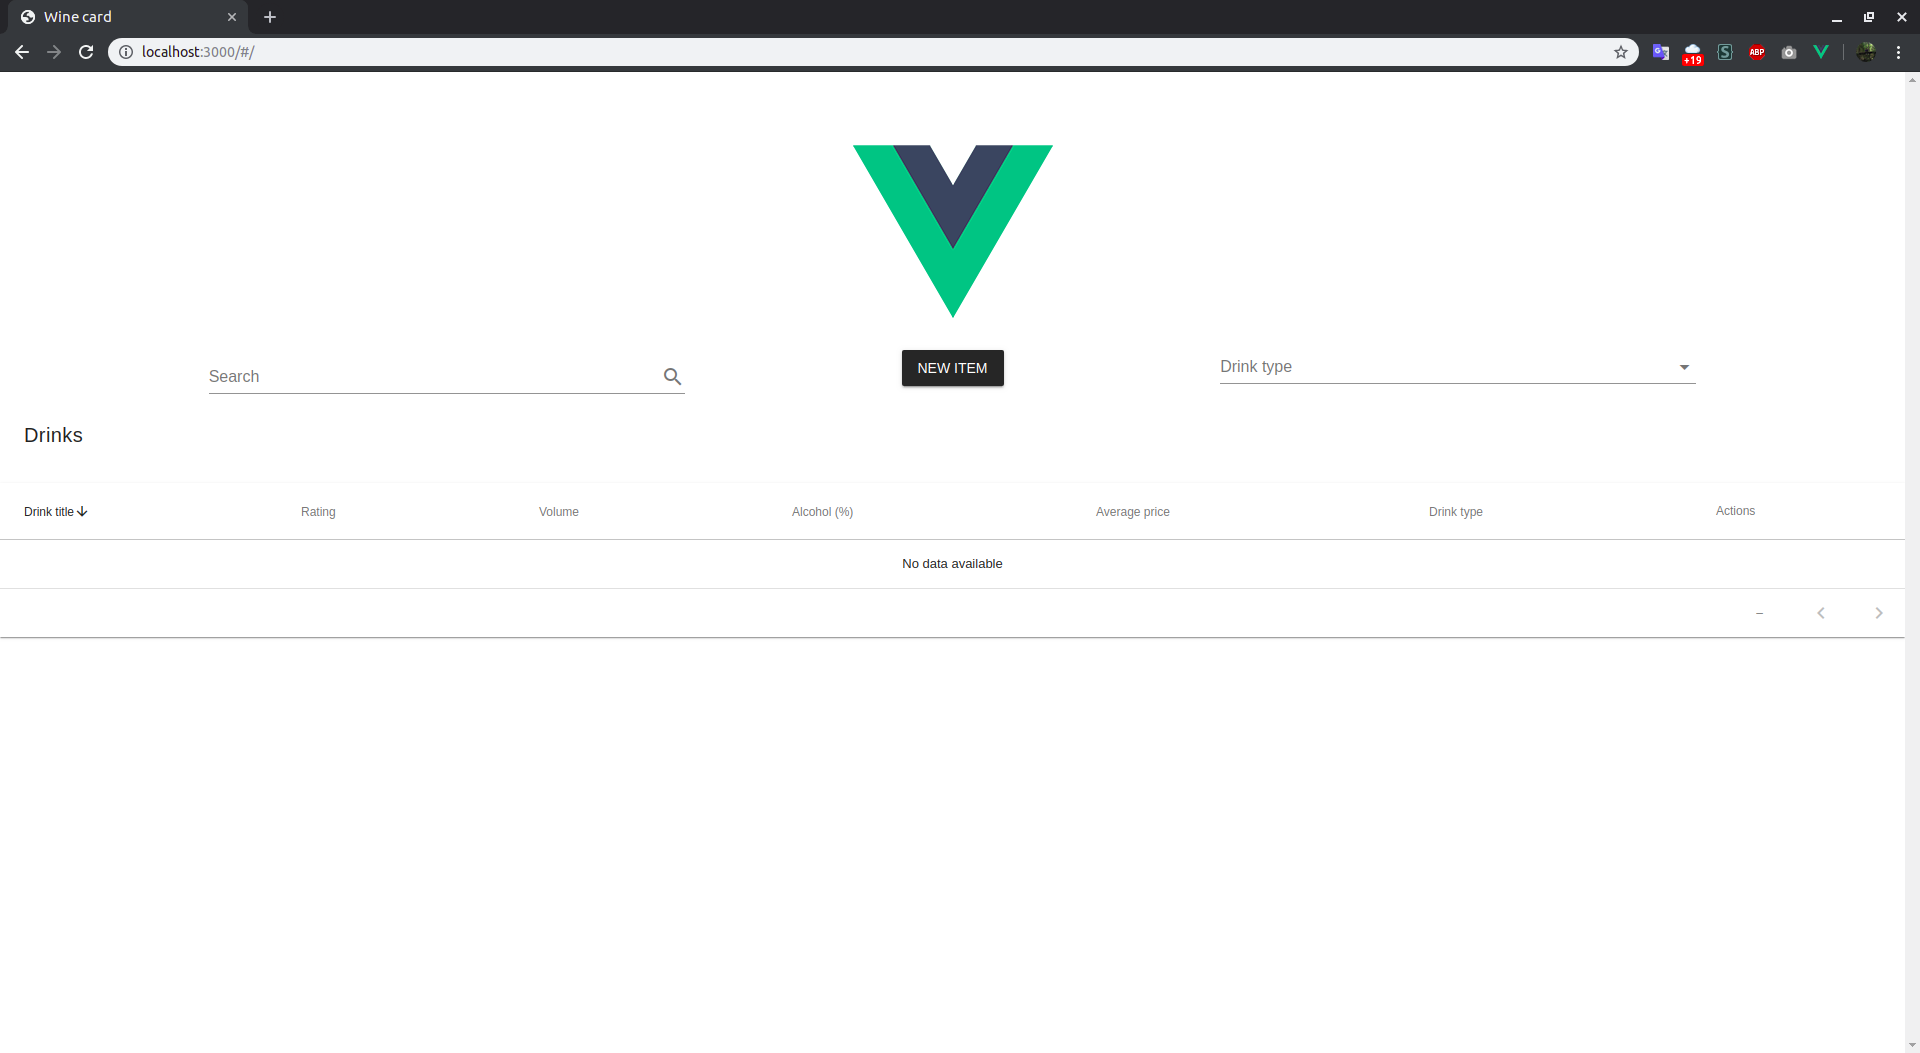
\includegraphics[scale=0.24]{index1}
		\caption{Начальная страница} 
		\label{pic:1} % название для ссылок внутри кода
	\end{center}
\end{figure}

При нажатии на кнопку "V" пользователь получает список всевозможных напитков из таблицы drinks:

\begin{figure}[H]
	\begin{center}
		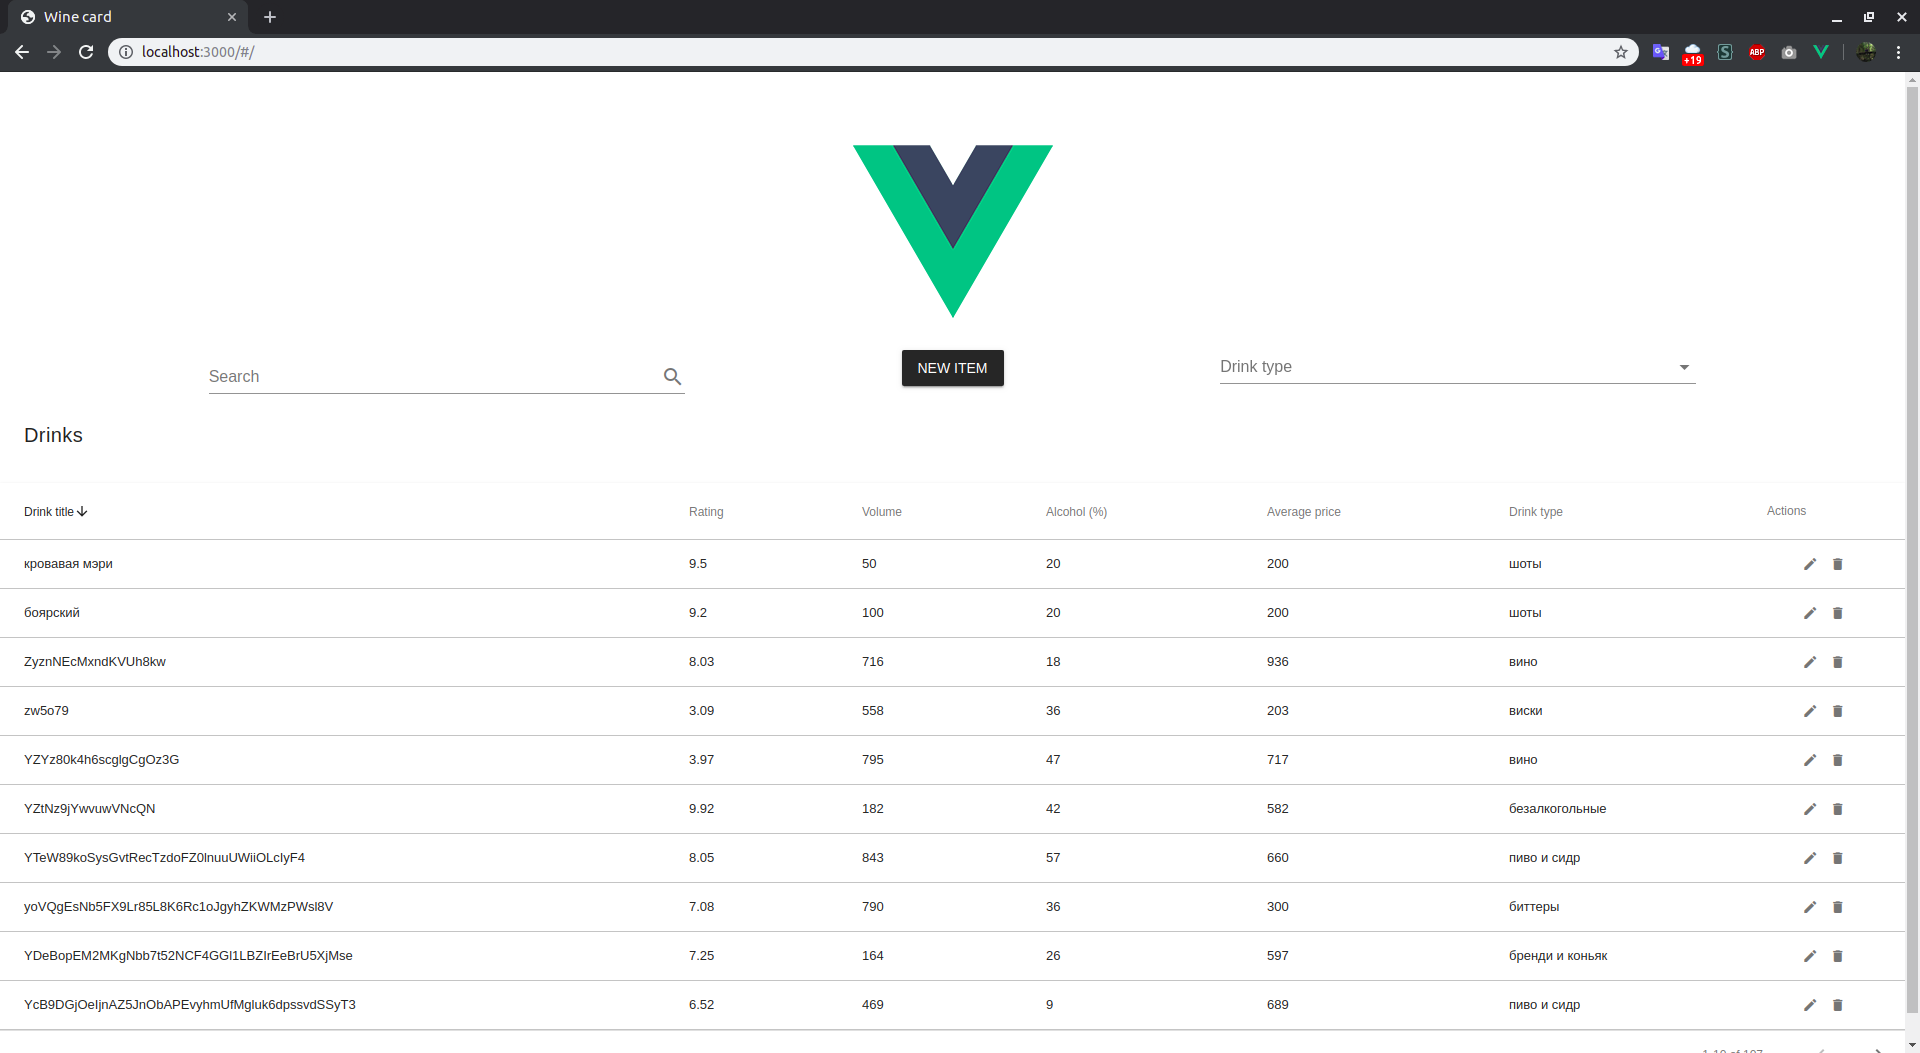
\includegraphics[scale=0.24]{index2}
		\caption{Начальная страница после нажатия на кнопку "V"} 
		\label{pic:2} % название для ссылок внутри кода
	\end{center}
\end{figure}

Далее, в строке поиска, пользователь может искать информацию о напитке по его названию.

С помощью кнопки "New item" пользователь может добавить новый напиток в таблицу, указав в модальном окне его параметры:

\begin{figure}[H]
	\begin{center}
		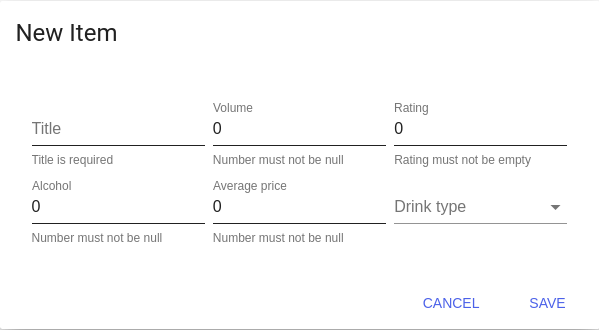
\includegraphics[scale=0.25]{newItem}
		\caption{Окно добавления нового напитка} 
		\label{pic:3} % название для ссылок внутри кода
	\end{center}
\end{figure}

При добавлении нового напитка или изменения имеющегося проходит валидация вводимых/изменяемых данных.
Осуществляется проверка на то, не являются ли строки пустыми. Для поля title стоит ограничение в 50 символов. Поля, содержащие числовые значения также проверяются. Значения должны быть > 0. Поле rating должно быть <= 10.

При введении некорректных данных, пользователь не сможет нажать на кнопку "Save" и совершить запрос к серверу.

С помощью нажатия на поле "Drink type" пользователь может из всплывающего списка выбрать тип напитка и отобразить напитки только этого типа:

\begin{figure}[H]
	\begin{center}
		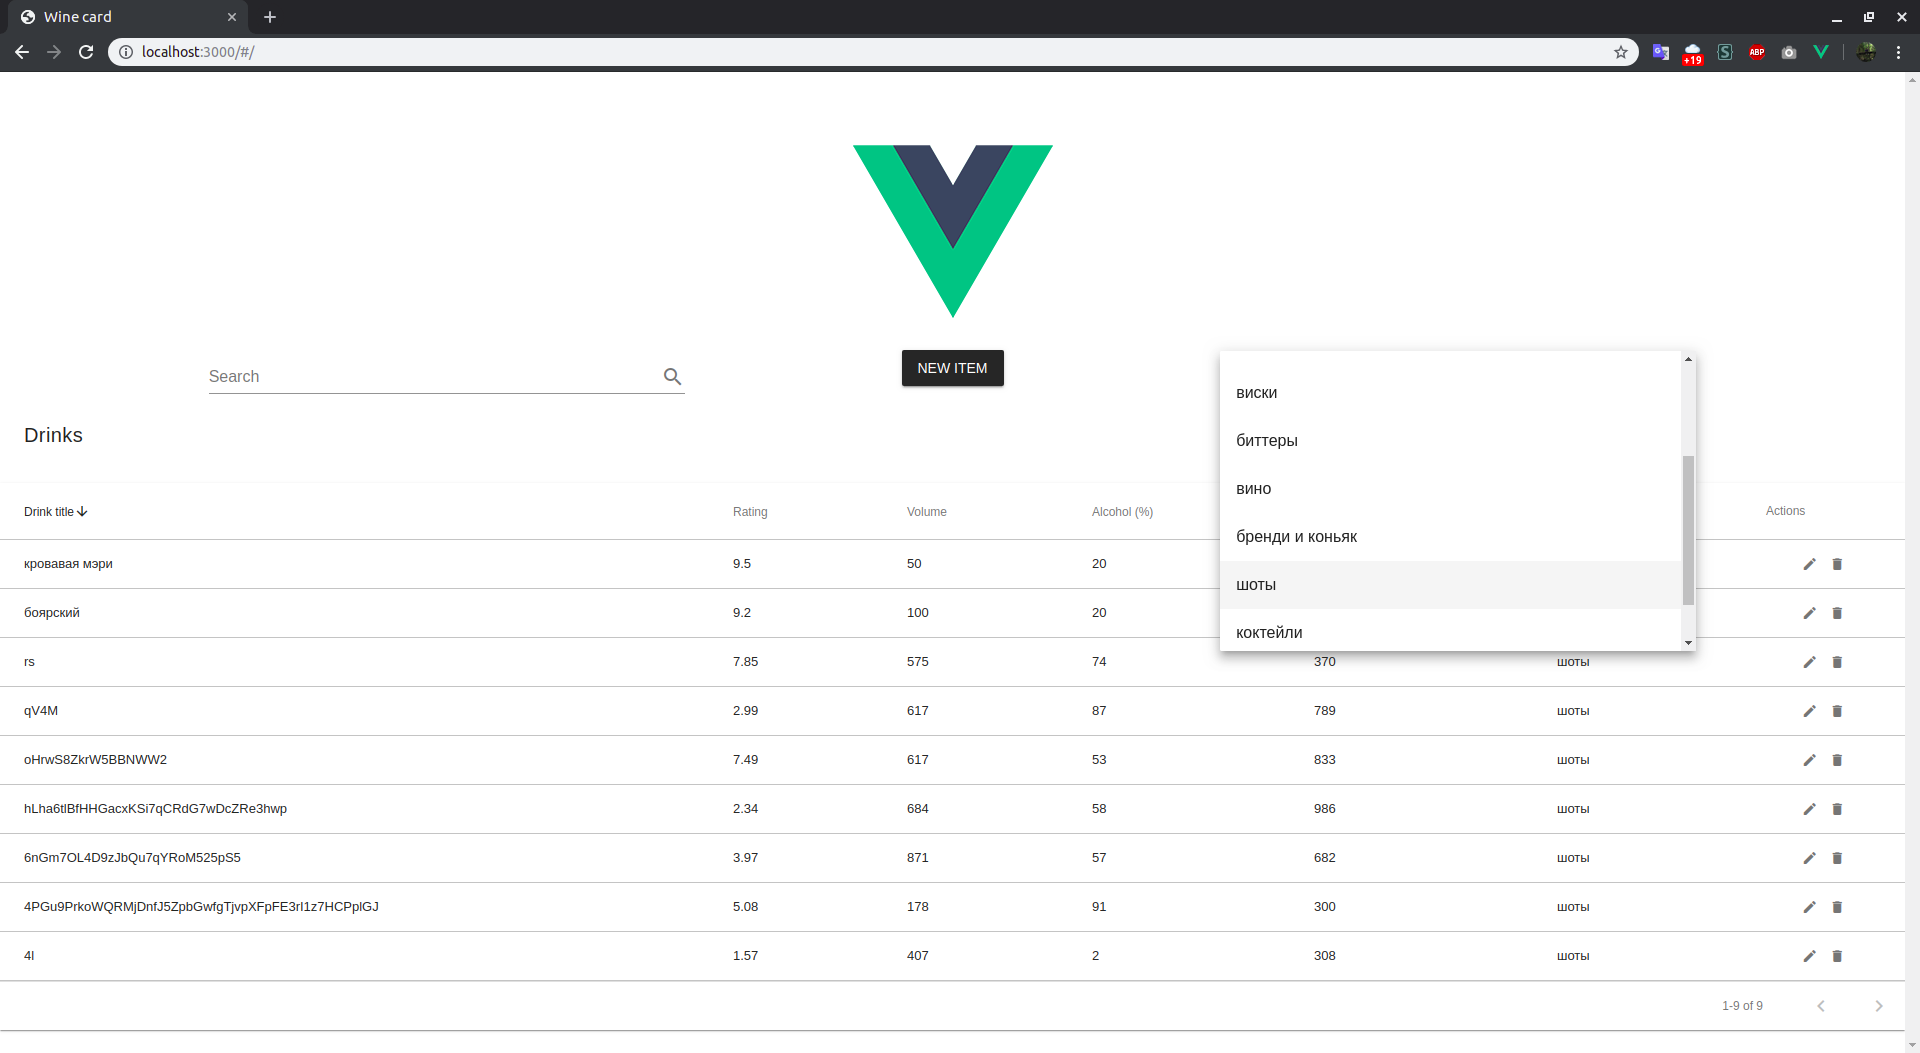
\includegraphics[scale=0.25]{sort}
		\caption{Сортировка по типу напитка} 
		\label{pic:4} % название для ссылок внутри кода
	\end{center}
\end{figure}

Если нажать на один из напитков, раскроется информация о том, из каких компонентов он состоит и где можно его выпить:

\begin{figure}[H]
	\begin{center}
		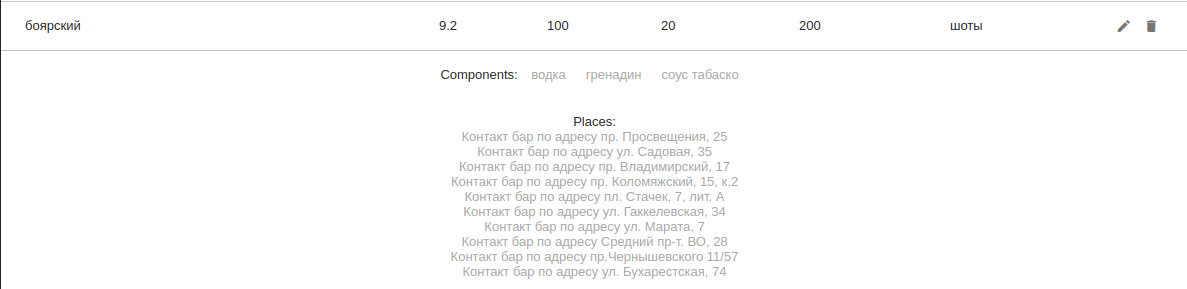
\includegraphics[scale=0.4]{inf}
		\caption{Дополнительная информация о напитке} 
		\label{pic:5} % название для ссылок внутри кода
	\end{center}
\end{figure}

Также, пользователь может отредактировать или удалить существующую позицию из таблицы с помощью иконок, расположенных справа.

\section{Вывод}
В данной курсовой работе мной было реализовано web-приложение, позволяющее через пользовательский интерфейс взаимодействовать с моей БД "wine\_card". Мной были использованы
изученные мной ранее в семестре хранимые процедуры и триггеры, а также более детально
изучена работа с форматом json.
Правильность работы моего приложения была протестирована c помощью функционального тестирования.
\end{document}
